\chapter{Implementation}
\label{sec:implementation}


\section{Frontend}
\subsection{Architecture}
\begin{figure}[h]
\centering
\begin{forest}
  for tree={
    font=\ttfamily\small,
    grow'=0,
    child anchor=west,
    parent anchor=south,
    anchor=west,
    calign=first,
    inner xsep=4pt,
    edge path={
      \noexpand\path [draw, \forestoption{edge}]
        (!u.south west) +(7.5pt,0) |- (.child anchor)\forestoption{edge label};
    },
    before typesetting nodes={
      if n=1{insert before={[,phantom]}}{},
    },
    fit=band,
    before computing xy={l=15pt},
  }
  [frontend/
    [api/
      [base.js]
      [documents.api.js]
      [models.api.js]
      [projects.api.js]
      [document-model-links.api.js]
      [{stats.api.js, logs.api.js}]
    ]
    [modules/
      [document/
        [file.js]
        [selection.js]
      ]
      [model/
        [wfadaptor.js]
        [endpoints/]
        [themes/]
        [utils/]
      ]
    ]
    [pages/
      [home/
        [init.js]
        [ui/
          [projects.ui.js]
          [project-creation.ui.js]
          [dashboard.ui.js]
        ]
      ]
      [stats/
        [init.js]
        [store.js]
        [ui/]
      ]
      [workspace/
        [init.js]
        [services/
          [workspace.service.js]
          [document.service.js]
          [model.service.js]
        ]
        [store/
          [workspace.store.js]
          [documents.store.js]
          [document-viewer.store.js]
          [models.store.js]
          [model-editor.store.js]
          [project-graph.store.js]
        ]
        [ui/]
        [utils/]
        [css/]
      ]
    ]
    [shared/
      [utils/
        [{url.js, dom.js, date.js}]
        [{store.js, ui.js, number.js}]
      ]
      [widgets/
        [inline-editor.js]
        [version-selector.js]
        [version-tag.js]
      ]
    ]
    [{index.html, workspace.html}]
    [{stats.html, document-viewer.html, model-viewer.html}]
    [constants.js]
  ]
\end{forest}
\caption{Frontend directory structure of the DBPM application.}
\label{fig:frontend_structure}
\end{figure}

\section{Backend}
\subsection{Architecture}
The backend is using Fastify, as its out-of-box support for schame validation. As shown in the figure~\ref{fig:imp_backend_schema_example}, the example code snippet of the backend
\begin{lstlisting}[language=Python]
\label{fig:imp_backend_schema_example}
def hello():
    print("Hello World")
\end{lstlisting}
The backend implemention follows the layered Controller-Service-Repository architecture.
\begin{figure}[H]
    \centering
    \caption{Backend Component} 
    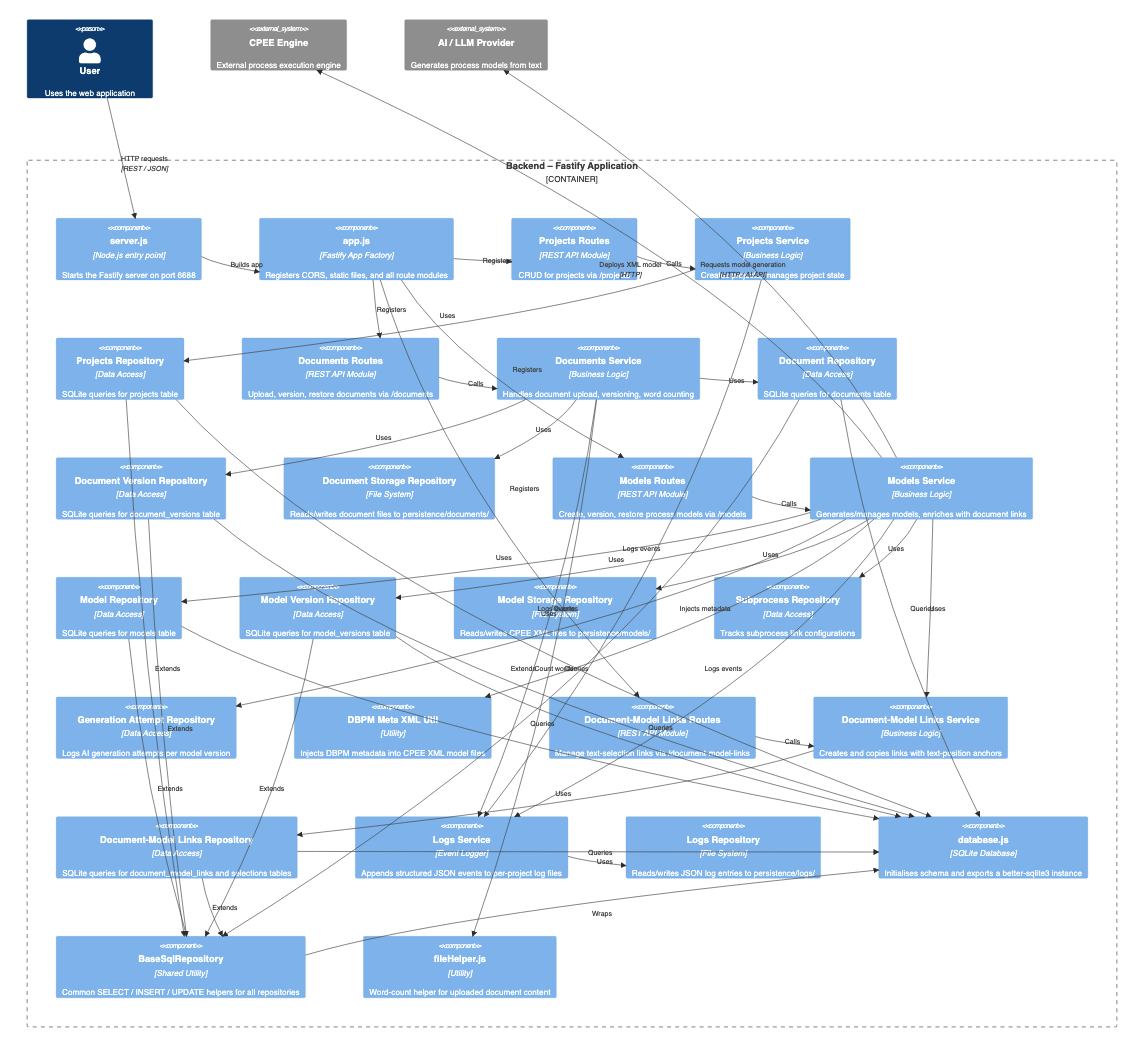
\includegraphics[width=0.8\textwidth]{images/imp_backend_com.png}
    \floatfoot{The backend component of the document-based process modeling tool.}
    \label{fig:imp_backend_com}
\end{figure}
